\chapter{MIP Timing Detector (MTD)}
\section{Introduction}

In the coming years the LHC will be working toward upgrades that will lead a substantial increase in luminosity.  The timeline for future operations of the LHC is shown in Figure \ref{fig:lhctimeline}.  In 2019 the LHC entered a two-year shutdown, Long Shutdown 2 (LS2).  Upgrades of the LHC injector complex to increase the beam brightness will take place during this shutdown.  After LS2 the LHC will enter Run 3 which will run for three years at 13-14 TeV.  At the completion of Run 3 the LHC will enter Long Shutdown 3 (LS3) which will last approximately 2.5 years.  During LS3 the optics in the interaction region will be upgraded to produce smaller beams at the interaction point.  The completion of this upgrade will usher in the High Luminosity (HL-LHC) era or Phase 2 of LHC operations, during which the combination of brighter beams and a new focusing scheme at the IP allows for a potential luminosity of 2x10$^{35}$ cm$^{-2}$s$^{-1}$ at the beginning of each fill \cite{Apollinari:2017cqg}.  

\begin{figure}[h]
	\centering
	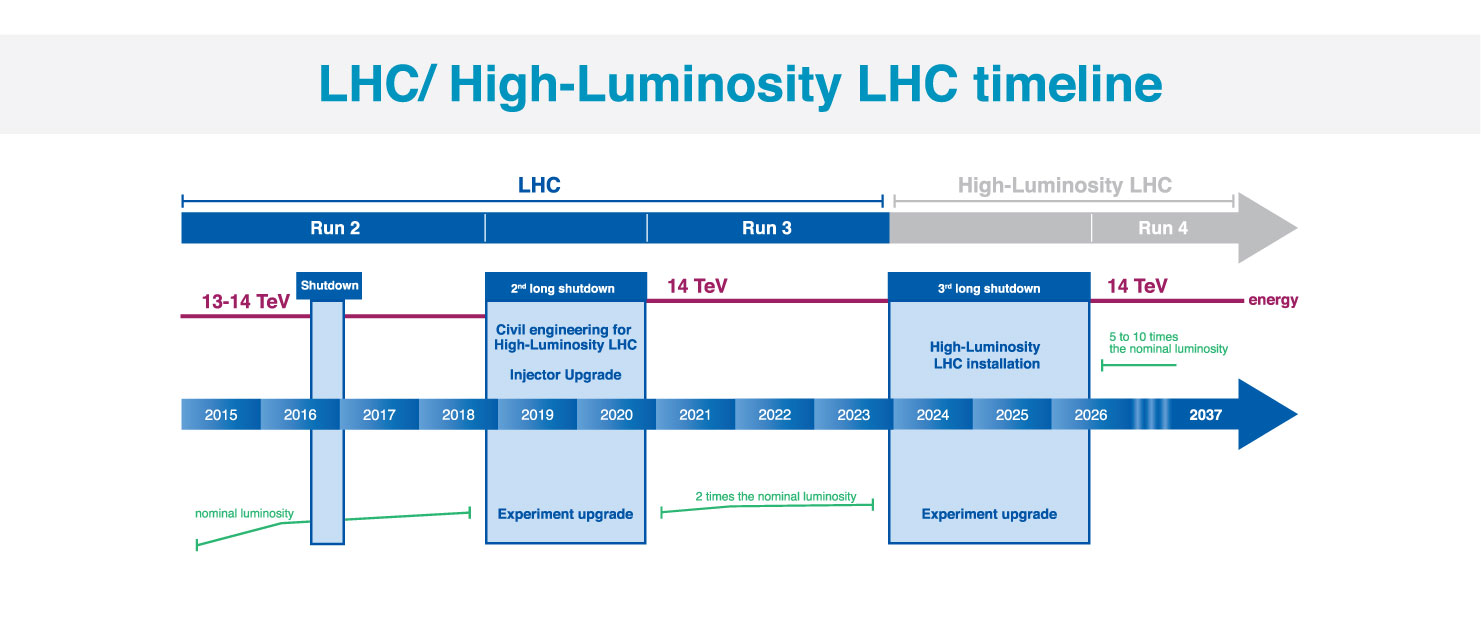
\includegraphics[width=1.0\linewidth]{Figures/LHCTimeline}
	\caption[Timeline for LHC]{Timeline for LHC \cite{DeMelis:2063307}}
	\label{fig:lhctimeline}
\end{figure}

The increased luminosity results in more interactions per bunch crossing or pileup.  In order to limit the amount of pileup the experiments must disentangle to more manageable levels, the nominal scenario would be operating at a stable luminosity of $5.0\times10^{34}$ cm$^{-2}$ s$^{-1}$.  This would limit the pileup to an average of 140.  The ultimate scenario for operations would be running at $7.5\times10^{34}$ cm$^{-2}$ s$^{-1}$ which brings the average pileup up to 200.  The CMS detector in its current state is not capable of dealing with $\approx$140-200 pileup.  At this level of pileup the spacial overlaps of tracks and energy depositions would lead to a degradation in the ability to identify and reconstruct hard interactions. In order to preserve the data quality of the current CMS detector this increased pileup must be reduced to an equivalent level approximately equal to current LHC operations which is $\sim$40.  The collision vertices within a bunch crossing have an RMS spread of 180-200 ps in time.  If the beam spot were to be sliced into consecutive snap shots of 30-40 ps then the pileup levels per snapshot would be approximately 40.  The space-time reconstruction of a 200 pileup event is shown in Figure \ref{fig:mtdpileup}.  The addition of timing information to the $z$ position spreads apart the vertices that would otherwise have been merged together and indiscernible.  In order to achieve this a detector dedicated to the precise timing of minimum ionizing particles (MIPs), the MTD, will be added to the CMS detector.  



\begin{figure}[h]
	\centering
	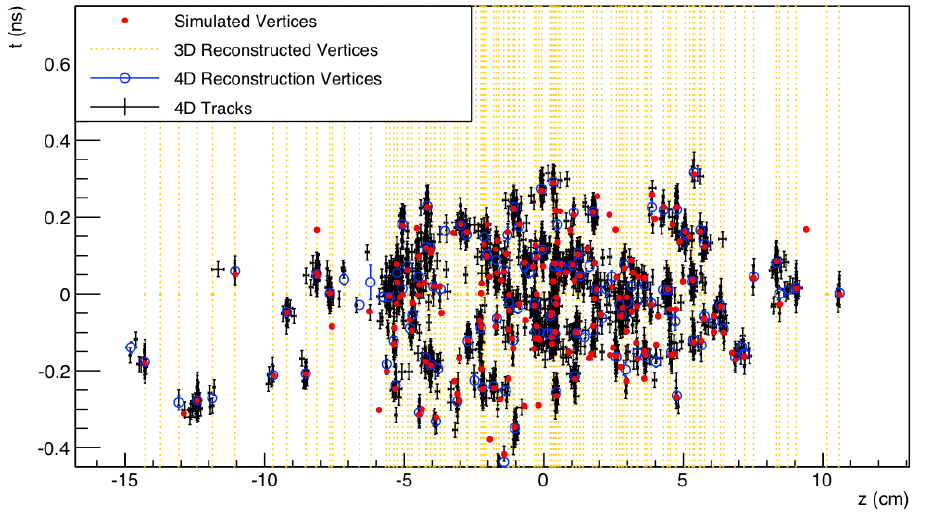
\includegraphics[width=1.0\linewidth]{Figures/MDT_pileup}
	\caption{Vertices from a simulated 200 pileup event with MTD timing resolution of $\sim$30 ps. The red dots represent the simulated vertices while the yellow lines indicate vertices reconstructed without the use of timing information. The black crosses and blue open circles represent tracks and vertices reconstructed using time information from the MTD. Reprint from}
	\label{fig:mdtpileup}
\end{figure}

\begin{figure}[h]
	\centering
	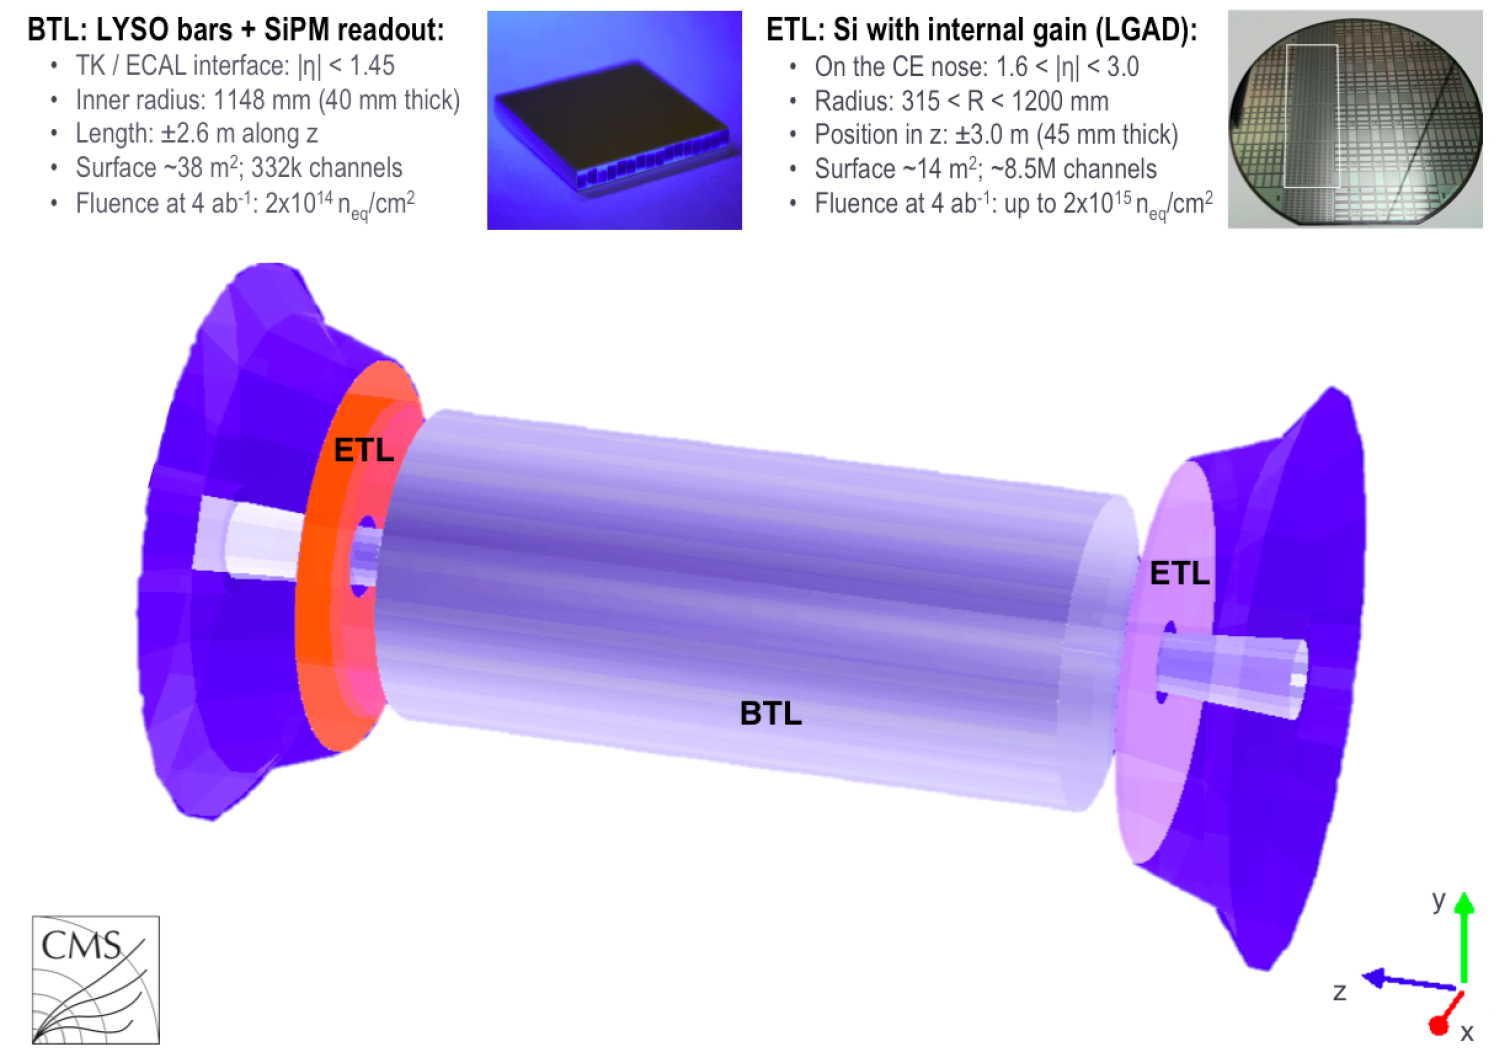
\includegraphics[width=1.0\linewidth]{Figures/MTD_overview}
	\caption[Schematic view of MTD]{Schematic view of the proposed MTD implemented in the GEANT simulation of the CMS detector. The central region makes up the BTL which will be located in the space between the tracker and the ECAL. The ETL will be located in front of the endcap calorimeter. Reprint from }
	\label{fig:mtdoverview}
\end{figure}


%The MTD will provide timing information with a resolution of 30-40 ps at the start of the HL-LHC era.  Radiation damage is expected to degrade this to 50-60 ps by the end of the HL-LHC era.


\section{Barrel Timing Layer}
 The Barrel Timing Layer (BTL) makes up the barrel region of the MTD.  It will provide pseudorapidity coverage up to $|\eta| = 1.48$ with a geometric acceptance of $\sim 90\%$.  The BTL will be capable of detecting MIPs with a time resolution of 30 ps at the start of Phase-2 operations and a luminosity-weighted time resolution of $\sim45$ ps when radiation damage effects are taken into account.     
 
 The fundamental element for MIP detection in the BTL is a thin scintillating bar made of Lutetium Yttrium Orthosilicate crystals doped with Cerium ($(Lu_{1-X}Y_X)_2SiO_5:Ce$) which is referred to as LYSO:Ce.  The bars are 57 mm long, 3.12 mm wide, and have an average thickness of 3 mm.  A silicon photomultiplier (SiPM) is attached to each end of the LYSO:Ce bar.  This double-ended readout gives uniform time response along the length of the crystal by eliminating the time delay effect from light propagating along the crystal and the ability to extract positional information for tracking. 
 
 An overview of the BTL and its components is shown in Figure \ref{fig:btloverview}.  The longitudinal axis of each crystal bar is oriented along the $\phi$-direction in the CMS detector.  The crystals are grouped in 1 $\times$ 16 ($\phi \times z$) arrays that each form a \textit{module}.  Each \textit{module} has 32 SiPMs (2 for each bar) resulting in 32 readout channels.  These \textit{modules} are then grouped in a 3 $\times$ 8 ($\phi \times z$) arrangement to make up a readout unit (RU) as shown in Figure \ref{fig:btlreadoutunit}.  Each \textit{module} is read out by a dedicated ASIC called the TOFHIR (Time-of-flight, High Rate) chip which is capable of reading out 32 channels at a time.  The TOFHIR chip gives precision timing information using discrimination of the leading edge of pulses from the SiPMs followed by a time-to-digital converter (TDC).  When using discrimination techniques like this the time for a pulse to cross the discriminating threshold depends on the height of the pulse.  This results in an amplitude-dependent timing variation called time walk.  In order to correct for this time walk effect the ASIC also measures pulse amplitude. Six ASICs are mounted on each of four front-end boards (FEBs) on a RU giving a total of 24 ASICs and 768 SiPMs per RU.  The RUs are then arranged in trays along the $z$-direction.  Each tray holds six RUs, runs along half the length of the detector, and spans $10^\circ$ along $\phi$.  To summarize, a total of 72 trays (36 azmuthal sections each split into a $+z$ and $-z$ section) contain 331776 SiPMs and 165888 LYSO:Ce bars.  This gives a detector granularity that has an average occupancy of about 7\% at 200 pileup, which limits the likelihood of multiple hits within a single crystal during a bunch crossing.  
 
 In order to have a negligible impact on the energy resolution of the ECAL, the thickness of the LYSO:Ce crystals is varied along the $z$-axis of the detector.  This variation is done in three sections such that the thickness of material is as uniform as possible while not exceeding 0.4 $X_0$ where $X_0$ is one radiation length.  This is done in three sections as a function of $\eta$
 
 
 \begin{figure}[h]
 	\centering
 	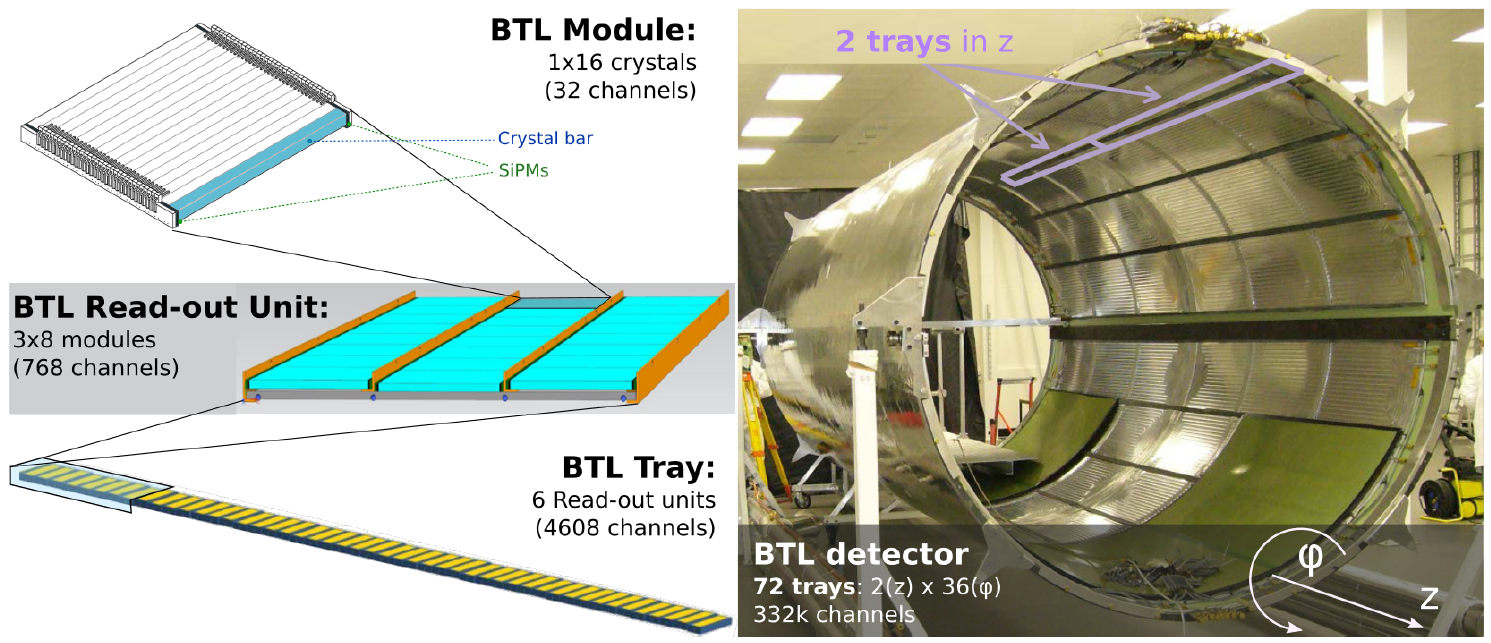
\includegraphics[width=1.0\linewidth]{Figures/BTL_overview}
 	\caption[Overview of the BTL]{On the left is an overview showing how the various components of the BTL fit together into modules, read-out units, and trays.  On the right is a view of how the trays will fit into the Tracker Support Tube (TST)}
 	\label{fig:btloverview}
 \end{figure}
 

\begin{figure}[h]
	\centering
	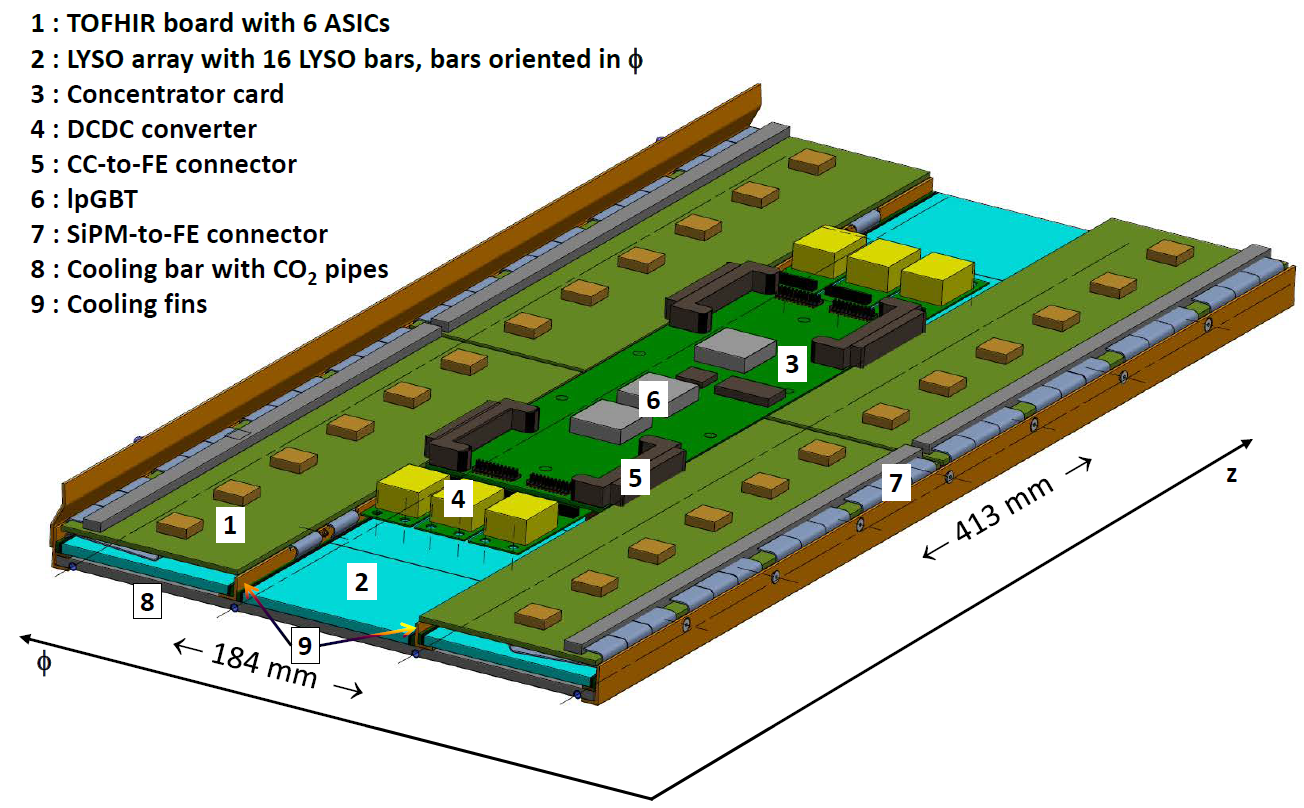
\includegraphics[width=1.0\linewidth]{Figures/BTL_readoutunit}
	\caption[Readout unit for the BTL.]{Readout unit for the BTL.}
	\label{fig:btlreadoutunit}
\end{figure}


\subsection{LYSO:Ce crystals}


\subsection{SiPMs}


\subsection{Glue qualification}



%As mentioned above, the fundamental active element in the BTL is a thin scintillating bar made of Lutetium Yttrium Orthosilicate crystals doped with Cerium ($(Lu_{1-X}Y_X)_2SiO_5:Ce$) which is referred to as LYSO:Ce.  The bars are 57 mm long, 3.12 mm wide, and have an average thickness of 3 mm.  A silicon photomultiplier (SiPM) is attached to each end of the LYSO:Ce bar.  This double-ended readout gives uniform time response along the length of the crystal and the ability to extract positional information for tracking.  


